\section{Examples}

Consider the case of an analyst looking to explore the sources and causes of
polling error in a presidential election. One hypothesis \cite{zukin2015s}
is that the rapid switch from landlines to cellphones increases the
difficulty of contacting potential poll respondents. The analyst may
begin her analysis by comparing the polling error in a state with the
distribution of households with landlines, for the set of states for which
polling error was most pronounced. In order to probe deeply, the analyst
accesses a household-level survey that includes data on
whether the household has a landline. One such survey --- which will be
discussed further (Sec~\ref{subsec:datasets}) --- is the American Community Survey (ACS),
conducted by the US Census Bureau.

Surveys are rife with missing values due to non-response and other issues, and
the ACS is no exception. The Census Bureau and other similar organization attempt to present
data in as unadulterated a fashion as possible. The ACS dataset is not amenable to one-time
imputation by either the Census Bureau, for this reason, or the analyst's organization,
which likely uses the same database for a variety of unrelated uses (asking for different
imputation strategies). Thus, the analyst must deal with missing values in one way or
another.

In this case, a non-negligible fraction of respondents omitted information on whether they
have a landline. The analyst hypothesizes that older houses are more likely to have
landlines and that households that are relatively new are less likely to have landlines. 
The analyst could take advantage of these presumed correlations to impute the missing values
on the base table in one expensive operation. On the other hand, the query could be run
directly and rows with missing values may be dropped entirely. With ImputeDB, the analyst
could impute the relevant subset of data on-the-fly, achieving better performance without
losing the information in the dropped examples.

The analyst submits a query (Figure~\ref{fig:example-query}) to ImputeDB which finds an optimized query
plan\footnote{The analyst specifies a relatively high value of $\alpha$, the quality
emphasis parameter, in order to receive a plan that does an expensive imputation step. See
Section~\ref{sec:cost-model} for more details.}. The resulting query plan
(Figure~\ref{fig:query-plan})
imputes missing values for \verb!acs.TEL! after states with high polling error have been
selected. This decision reduces the set of tuples that must be input into the imputation
algorithm to just those that are relevant to the query. Later, we show the algorithms that
the ImputeDB query optimizer uses in order to detect these opportunities and control the
tradeoffs between efficiency and imputation quality. Finally, note that the optimizer doesn't
place any imputation operator for the \verb|acs.ST| column, as optimizer uses the histogram to
detect that there are no missing values there (as might be expected for a survey question that isn't
impacted by non-responses).

\begin{figure}
\begin{lstlisting}[language=SQL]
SELECT polling.ST, AVG(acs.TEL)
FROM polling, acs
WHERE polling.ST = acs.ST
  AND polling.ERROR > 50         -- 5 percentage points
GROUP BY polling.ST;
\end{lstlisting}
\caption{A typical analyst query on ACS data}
\label{fig:example-query}
\end{figure}

\begin{figure}[!ht]
    \centering
    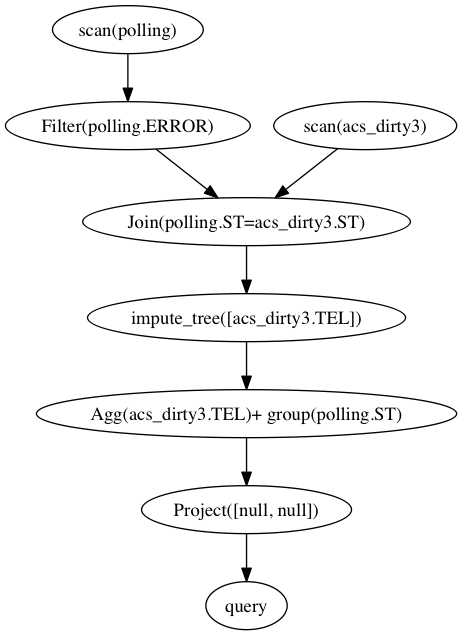
\includegraphics[width=0.6\textwidth]{figures/example.png}
    \caption{Query plan generated by ImputeDB prioritizing imputation quality}
    \label{fig:query-plan}
\end{figure}
        
%%% Local Variables:
%%% mode: latex
%%% TeX-master: "main"
%%% End:
